\documentclass[runningheads]{llncs}

\usepackage{graphicx}
\usepackage{amsmath,amssymb,amsfonts}
\usepackage{algorithmic}
\usepackage{textcomp}
\usepackage{xcolor}
\usepackage{url}
\usepackage{booktabs}
\usepackage{array}
\usepackage{multirow}
\usepackage{float}
\usepackage{subcaption}
\usepackage{stfloats}
\usepackage{placeins}
\usepackage{enumitem}
\setlist{nosep}
\usepackage{caption}
\captionsetup[figure]{font=small,skip=2pt}
\captionsetup[subcaption]{font=small,skip=1pt}

% Reduce spacing around equations
\setlength{\abovedisplayskip}{6pt}
\setlength{\belowdisplayskip}{6pt}
\setlength{\abovedisplayshortskip}{3pt}
\setlength{\belowdisplayshortskip}{3pt}

% Reduce spacing around floats (figures/tables)
\setlength{\textfloatsep}{8pt plus 2pt minus 2pt}
\setlength{\floatsep}{8pt plus 2pt minus 2pt}
\setlength{\intextsep}{6pt plus 2pt minus 2pt}
\setlength{\dbltextfloatsep}{8pt plus 2pt minus 2pt}
\setlength{\dblfloatsep}{8pt plus 2pt minus 2pt}

\begin{document}

\titlerunning{Bridging the Generalization Gap in Deepfake Detection}
\authorrunning{E. S. Pokharia et al.}

\title{Bridging the Generalization Gap in Deepfake Detection: Ensemble and Hybrid Strategies for Cross-Domain Robustness}

\author{Eeshan Singh Pokharia\inst{1}\orcidID{} \and
Soumya Mukherjee\inst{1}\orcidID{} \and
Jayendra Singh\inst{1}\orcidID{} \and
Manoj Patra\inst{2}\orcidID{} \and
Ankit Jain\inst{1}\orcidID{} \and
Shiv Prasad\inst{1}\orcidID{}}

\institute{Department of Computer and Communication Engineering,
The LNM Institute of Information and Technology, Jaipur, India\\
\email{\{23ucc540,soumya.mukherjee,ankit.jain,psad.shiv\}@lnmiit.ac.in}
\and
Department of Computer Science and Engineering,
National Institute of Technology, Warangal, India}

\maketitle

\begin{abstract}
While Convolutional Neural Networks (CNNs) achieve near-perfect accuracy on deepfake detection benchmarks, they suffer from a severe ``generalization gap'' when evaluated on datasets with unseen manipulation techniques, and exhibit extreme brittleness under adversarial attacks. In this study, the authors systematically address these limitations by introducing and evaluating three advanced paradigms: a Multi-Scale Feature Fusion CNN, a Hybrid CNN-Transformer architecture, and a Frequency-Aware dual-branch network. Furthermore, the investigation includes the efficacy of ensemble methods---including Hard Voting, Soft Voting, and Learned Logistic Stacking---across six distinct model combinations. Using the Celeb-DF dataset for training and FaceForensics++ for cross-dataset evaluation, this work advances the state-of-the-art in-distribution performance to 99.51\% accuracy and 99.80\% AUC via a 5-model Soft-Voting Ensemble. Extensive adversarial evaluations using FGSM and PGD attacks reveal a critical and previously unreported insight: the Vision Transformer exhibits \textit{complete adversarial immunity} in accuracy, maintaining exactly 63.54\% across all perturbation budgets ($\epsilon \in [0.01, 0.10]$), while models maximizing in-distribution accuracy (EfficientNet-B0, ResNet50) collapse to 0\% under PGD ($\epsilon=0.05$). XceptionNet similarly demonstrates natural robustness ($\sim$56\% under PGD). These findings demonstrate that the generalization gap is fundamentally architectural: bridging it requires moving beyond purely spatial CNNs toward structurally hardened architectures.
\end{abstract}

\keywords{deepfake detection \and adversarial robustness \and cross-dataset evaluation \and vision transformers \and frequency-domain analysis \and ensemble learning}

\section{Introduction}
The democratization of synthetic media tools has accelerated the generation of hyper-realistic deepfakes, posing escalating threats to digital identity, political integrity, and evidence authentication. Modern deepfake detectors principally leverage deep Convolutional Neural Networks (CNNs) to parse microscopic spatial inconsistencies. However, a critical \textit{generalization gap} persists: a model perfectly optimized for one dataset often fails catastrophically on videos generated by an unseen GAN or blending algorithm~\cite{cross_dataset}.

The FaceForensics++ benchmark~\cite{faceforensics} standardized evaluation across multiple manipulation techniques, enabling systematic comparison of detection architectures. As the field matured, XceptionNet~\cite{xception} with depthwise separable convolutions, EfficientNet~\cite{efficientnet} using compound scaling, and ResNet~\cite{resnet} with residual connections became dominant baselines. More recently, Vision Transformers (ViT)~\cite{vit} have been adapted for visual tasks by processing images as patch sequences with global self-attention, offering fundamentally different inductive biases than CNNs.

In a preceding comparative study, it was established that while architectures like EfficientNet-B0 achieve $\sim$99\% in-distribution accuracy on Celeb-DF, their accuracy plunges to $\sim$50\% on FaceForensics++. This indicates that standard CNNs overfit to dataset-specific generation fingerprints rather than learning universal manipulation semantics. Furthermore, real-world deepfake detectors face the existential threat of adversarial perturbations---intentional pixel-level noise designed to fool classifiers---an area largely overlooked in standard benchmarking.

This paper systematically addresses the generalization and robustness gap through four interconnected strategies:
\begin{enumerate}
    \item \textbf{Hybrid CNN-Transformer:} Combining EfficientNet-B0's local texture extraction with Transformer self-attention for simultaneous local-global reasoning.
    \item \textbf{Multi-Scale Feature Fusion:} Aggregating features from four intermediate EfficientNet layers to capture artifacts across semantic granularities.
    \item \textbf{Ensemble Learning:} Investigation of Hard Voting, Soft Voting, and Learned Stacking across six distinct model combinations to mathematically marginalize individual architectural biases.
    \item \textbf{Frequency-Aware Dual-Branch CNN:} Processing the 2D-FFT magnitude spectrum alongside spatial features, exploiting spectral fingerprints left by GAN upsampling~\cite{frequency_analysis}.
\end{enumerate}

\section{Contributions}
This work advances the field through the following contributions:
\begin{enumerate}
    \item Recognition and design of three novel architectures---Hybrid CNN-Transformer (30.7M parameters), Multi-Scale Feature Fusion (\textbf{4.2M parameters}), and Frequency-Aware CNN (5.5M parameters)---pushing in-distribution AUC to 99.84\%.
    \item The most comprehensive ensemble ablation in deepfake detection literature: 6 model combinations $\times$ 3 aggregation strategies, establishing a new performance ceiling of 99.51\% accuracy via Soft-Voting.
    \item Rigorous adversarial evaluation (FGSM and PGD) across all 7 architectures at 5 perturbation budgets, revealing that Vision Transformers exhibit \textit{complete accuracy invariance} under both attack types.
    \item Comprehensive cross-dataset evaluation on FaceForensics++ and failure analysis via Grad-CAM across all 7 models on 20 verification images, identifying shared blindspots.
\end{enumerate}

\section{Methodology}

\subsection{Datasets and Preprocessing}
Training was conducted on \textbf{Celeb-DF (v2)}~\cite{cross_dataset} (18,472 images: 1,736 real, 16,736 fake; 80-10-10 split) and cross-dataset generalization was evaluated on \textbf{FaceForensics++}~\cite{faceforensics} (20,781 frames: 2,992 real, 17,789 fake). Frames were sampled at regular intervals, faces were localized via Haar Cascade with a 20\% margin, and crops were resized to $224 \times 224$ with $[0,1]$ normalization.

\subsection{Novel Architectural Paradigms}

\begin{figure*}[!htbp]
\centering
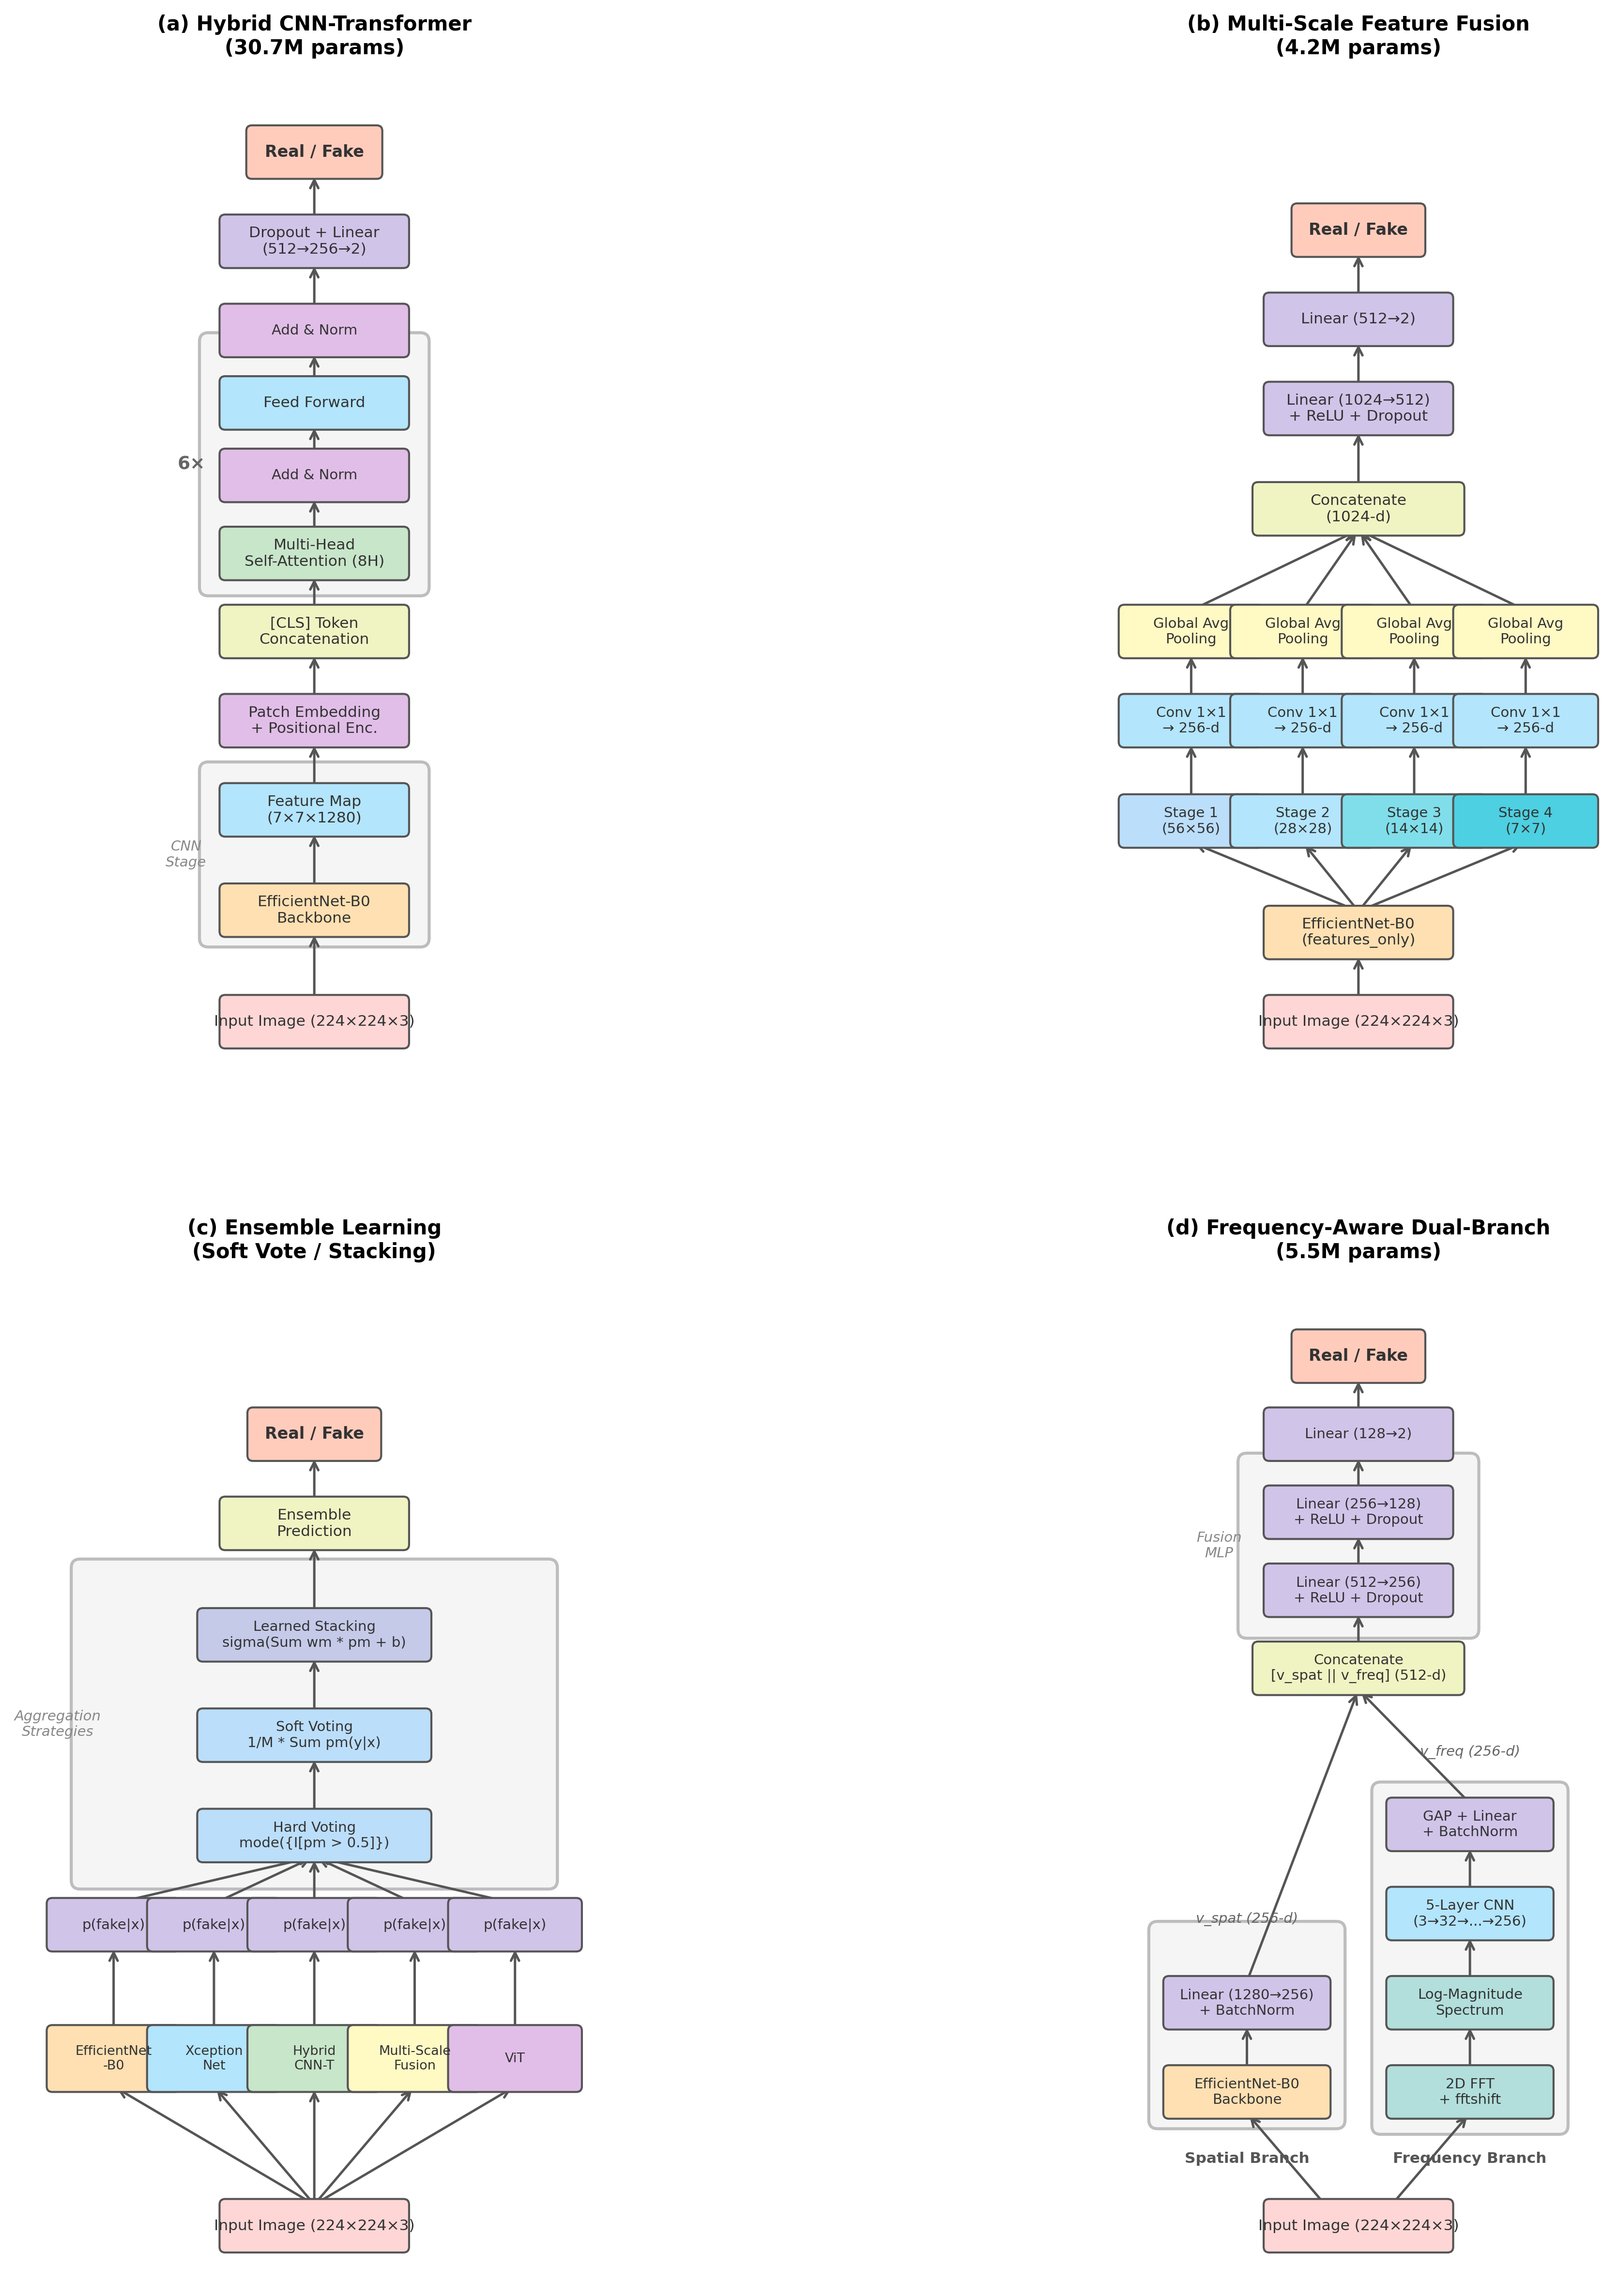
\includegraphics[width=0.95\textwidth]{figures/architecture_diagrams.png}
\caption{Architecture diagrams of the four novel detection paradigms. (a) Hybrid CNN-Transformer combining EfficientNet-B0 with 6-layer Transformer encoder. (b) Multi-Scale Feature Fusion aggregating four EfficientNet stages. (c) Ensemble Learning with three aggregation strategies. (d) Frequency-Aware Dual-Branch network processing spatial and FFT features in parallel.}
\label{fig:architectures}
\end{figure*}

\subsubsection{Hybrid CNN-Transformer.}
Standard CNNs possess constrained receptive fields, limiting contextual reasoning across distant facial regions. The HybridCNNTransformer routes an image through an EfficientNet-B0 backbone yielding a feature map $\mathbf{A} \in \mathbb{R}^{7 \times 7 \times 1280}$. This map is projected via a learnable patch embedding layer into $N$ tokens of dimension $d$, enriched with positional encodings $\mathbf{E}_{pos}$, and propagated through 6 layers of Multi-Head Self-Attention (MSA) with 8 heads:
\begin{align}
    \mathbf{z}_0 &= [\mathbf{x}_{cls}; \mathbf{a}_1 \mathbf{W}_p; \ldots; \mathbf{a}_N \mathbf{W}_p] + \mathbf{E}_{pos} \\
    \mathbf{z}'_l &= \text{MSA}(\text{LN}(\mathbf{z}_{l-1})) + \mathbf{z}_{l-1} \\
    \mathbf{z}_l &= \text{MLP}(\text{LN}(\mathbf{z}'_l)) + \mathbf{z}'_l
\end{align}
where $\mathbf{W}_p$ is the patch projection matrix, $\mathbf{x}_{cls}$ is a learnable classification token, and LN denotes Layer Normalization. The final classification is derived from the $\mathbf{x}_{cls}$ output. This enables cross-referencing of spatial manipulation artifacts (e.g., lighting disparities across opposite facial regions). The architecture totals 30.7M parameters.

\subsubsection{Multi-Scale Feature Fusion.}
Manipulation artifacts span semantic granularities---from macro boundary blending to micro textural noise. The MultiScaleFeatureFusion model isolates feature representations $F_i$ from $K=4$ intermediate stages of an EfficientNet-B0 encoder (indices [1,2,3,4]). Each $F_i$ is projected to a 256-dimensional representation via $1\times1$ convolution, globally pooled, and concatenated:
\begin{equation}
    \mathbf{v}_{fuse} = \sigma \left( \mathbf{W}_{fuse} \begin{bmatrix}
        \text{GAP}(\text{Conv}_{1\times1}(F_1)) \\
        \vdots \\
        \text{GAP}(\text{Conv}_{1\times1}(F_K))
    \end{bmatrix} + b_{fuse} \right)
\end{equation}
where GAP denotes Global Average Pooling. This yields a compact model of only \textbf{4.2M parameters}---the lightest in this study---while capturing multi-resolution artifacts.

\subsubsection{Ensemble Learning Strategies.}
Given $M$ constituent models parameterized by $\theta_1, \ldots, \theta_M$, let $p_m(y|x; \theta_m)$ denote the predicted deepfake probability for input $x$. Three aggregation mechanisms are defined:
\begin{enumerate}
    \item \textbf{Hard Voting:} Majority consensus: $y_{ens} = \text{mode}(\{\mathbb{I}_{p_m > 0.5}\}_{m=1}^M)$.
    \item \textbf{Soft Voting:} Arithmetic mean of posterior probabilities:
    \begin{equation}
        P_{ens}(y|x) = \frac{1}{M}\sum_{m=1}^{M} p_m(y|x; \theta_m)
    \end{equation}
    \item \textbf{Learned Stacking:} A Logistic Regression meta-classifier trained on the predictions of the base models:
    \begin{equation}
        P_{stack}(y|x) = \sigma\left(\sum_{m=1}^{M} w_m \cdot p_m(y|x) + b \right)
    \end{equation}
    where $\sigma$ denotes the sigmoid function and weights $w_m$ are learned from out-of-fold predictions.
\end{enumerate}
Six ensemble configurations (detailed in Table~\ref{tab:ensemble}) were evaluated across all three methods.

\subsubsection{Frequency-Aware Dual-Branch Network.}
GAN upsampling introduces spectral artifacts imperceptible in the spatial domain~\cite{frequency_analysis}. The \texttt{FrequencyAwareCNN} processes images via two parallel branches:

\textbf{Frequency Branch:} Computes the 2D Discrete Fourier Transform:
\begin{equation}
    \mathcal{F}(u,v) = \sum_{x=0}^{H-1} \sum_{y=0}^{W-1} \mathbf{I}(x,y) \, e^{-j2\pi\left(\frac{ux}{H} + \frac{vy}{W}\right)}
\end{equation}
The log-magnitude spectrum $\mathbf{M}(u,v) = \log(1 + |\mathcal{F}(u,v)|)$ is centered via \texttt{fftshift} and processed by a 5-layer CNN ($3 \rightarrow 32 \rightarrow 64 \rightarrow 128 \rightarrow 256 \rightarrow 256$ channels) to yield $\mathbf{v}_{freq} \in \mathbb{R}^{256}$.

\textbf{Spatial Branch:} A pre-trained EfficientNet-B0 encoder yielding $\mathbf{v}_{spat} \in \mathbb{R}^{256}$.

The branches are late-fused via concatenation and classified through a fusion MLP with dropout ($p=0.3$):
$\mathbf{v}_{fuse} = [\mathbf{v}_{spat} \parallel \mathbf{v}_{freq}] \rightarrow \text{MLP} \rightarrow \hat{y}$.
The architecture totals 5.5M parameters.

\subsection{Adversarial Evaluation Framework}
To assess robustness against active evasion, white-box attacks were deployed at $L_\infty$ bounds of $\epsilon \in \{0.01, 0.02, 0.05, 0.10\}$:
\begin{enumerate}
    \item \textbf{Fast Gradient Sign Method (FGSM)~\cite{fgsm}:} A single-step perturbation:
    \begin{equation}
        x_{adv} = x + \epsilon \cdot \text{sgn}(\nabla_x \mathcal{L}(\theta, x, y))
    \end{equation}
    \item \textbf{Projected Gradient Descent (PGD)~\cite{pgd}:} A 10-step iterative attack with step size $\alpha = \epsilon/4$, randomly initialized within the $\epsilon$-ball:
    \begin{equation}
        x_{t+1} = \Pi_{\mathcal{B}_\epsilon(x)} \left( x_t + \alpha \cdot \text{sgn}(\nabla_{x_t} \mathcal{L}(\theta, x_t, y)) \right)
    \end{equation}
    where $\Pi_{\mathcal{B}_\epsilon(x)}$ projects onto the $\epsilon$-ball $\{x' : \|x' - x\|_\infty \leq \epsilon\}$.
\end{enumerate}
All evaluated samples were clamped to $[0, 1]$ following perturbation.

\subsection{Model Interpretability}
Gradient-weighted Class Activation Mapping (Grad-CAM) was employed to visualize each model's decision rationale. For a target class $c$ and feature map $A^k$ from the final convolutional layer:
\begin{equation}
    L_{CAM}^c = \text{ReLU}\left(\sum_k \underbrace{\frac{1}{Z} \sum_i \sum_j \frac{\partial y^c}{\partial A_{ij}^k}}_{\alpha_k^c} \cdot A^k \right)
\end{equation}
where $\alpha_k^c$ captures the importance of feature map $k$ for class $c$, and $Z = H \times W$ is a normalization constant.

\section{Training Configuration}
All models were trained uniformly for 30 epochs on Celeb-DF using Binary Cross-Entropy loss, optimized with AdamW ($\beta_1{=}0.9, \beta_2{=}0.999$, weight decay $10^{-2}$) and a Cosine Annealing learning rate schedule bounded between $\eta_{max}{=}10^{-4}$ and $\eta_{min}{=}10^{-6}$. Batch size was 32, with early stopping (patience 10--20 epochs) and mixed-precision training for efficiency.

\section{Results}

\subsection{In-Distribution Performance (Celeb-DF)}
Table~\ref{tab:celebd_results} summarizes performance on the Celeb-DF test set. All seven models plus the best ensemble are compared.

\begin{table}[H]
\caption{Performance Comparison and Parameter Efficiency on Celeb-DF Test Set}
\label{tab:celebd_results}
\centering
\small
\setlength{\tabcolsep}{5pt}
\begin{tabular}{lrcccc}
\toprule
\textbf{Model} & \textbf{Params} & \textbf{Acc.} & \textbf{AUC} & \textbf{Prec.} & \textbf{F1} \\
\midrule
EfficientNet-B0   & 5.3M  & 98.70\% & 99.54\% & 98.72\% & 98.71\% \\
XceptionNet       & 38.9M & 98.76\% & 98.57\% & 98.76\% & 98.76\% \\
ResNet50          & 25.6M & 98.22\% & 99.50\% & 98.21\% & 98.15\% \\
Vision Transformer & 86.6M & 90.54\% & 50.35\% & 81.98\% & 86.05\% \\
\midrule
Multi-Scale Fusion      & \textbf{4.2M} & 98.76\% & 99.63\% & 98.63\% & 98.81\% \\
Hybrid CNN-Transformer  & 30.7M & 98.59\% & 99.67\% & 98.70\% & 98.66\% \\
Frequency-Aware CNN     & 5.5M  & 99.03\% & \textbf{99.84\%} & 98.92\% & 99.11\% \\
\midrule
\textbf{Ensemble (Soft-Vote, 5M)} & \textit{---} & \textbf{99.51\%} & 99.80\% & 99.51\% & 99.51\% \\
\bottomrule
\end{tabular}
\end{table}

The \textbf{Frequency-Aware CNN} achieved the highest standalone AUC (99.84\%), demonstrating that spectral features capture highly discriminative in-distribution signals. Critically, both the Multi-Scale model (4.2M params) and the Frequency-Aware model (5.5M params) matched or exceeded the performance of architectures 7--17$\times$ larger (XceptionNet at 38.9M, ViT at 86.6M), demonstrating that parameter-efficient designs can achieve state-of-the-art detection.

\subsection{Ensemble Ablation Study}
Table~\ref{tab:ensemble} presents the systematic ensemble ablation. Six model combinations across three aggregation methods were evaluated on both datasets.

\begin{table}[H]
\caption{Ensemble Ablation: Soft-Voting Performance Across Configurations}
\label{tab:ensemble}
\centering
\small
\setlength{\tabcolsep}{4pt}
\begin{tabular}{llcccc}
\toprule
\textbf{Configuration} & \textbf{Models} & \textbf{CDF Acc.} & \textbf{CDF AUC} & \textbf{FF++ Acc.} & \textbf{FF++ AUC} \\
\midrule
CNN-Only        & Eff, Xce, Res               & 99.24\% & 99.82\% & 54.75\% & 72.57\% \\
CNN+ViT         & Eff, Xce, Res, ViT          & 99.19\% & 99.66\% & 56.56\% & 72.70\% \\
New Models      & Hyb, MS                     & 99.35\% & 99.81\% & 54.52\% & 70.97\% \\
Full 6-Model    & Eff, Xce, Res, ViT, Hyb, MS & 99.41\% & 99.83\% & 55.77\% & 72.97\% \\
EfficientNet+ViT & Eff, ViT                   & 98.92\% & 98.49\% & 52.26\% & 68.82\% \\
\textbf{All-Best (5M)} & \textbf{Eff, Xce, Hyb, MS, ViT}  & \textbf{99.51\%} & 99.80\% & 55.43\% & 71.59\% \\
\bottomrule
\end{tabular}
\end{table}

The \textbf{All-Best 5-model Soft-Vote} ensemble achieved the highest Celeb-DF accuracy (99.51\%), surpassing even the Full 6-Model ensemble (99.41\%). This indicates that including ResNet50 in the ensemble marginally degrades performance, likely due to its high correlation with EfficientNet's feature space. However, all ensemble strategies failed to meaningfully bridge the cross-dataset gap: the best FF++ accuracy was 56.56\% (CNN+ViT), confirming that ensemble diversity alone cannot overcome the fundamental domain shift.

\subsection{Cross-Dataset Generalization Gap (FaceForensics++)}
When frozen models were evaluated on FF++ (Table~\ref{tab:cross_dataset}), massive degradation occurred across all architectures.

\begin{table}[H]
\caption{Cross-Dataset Generalization: Celeb-DF $\rightarrow$ FaceForensics++}
\label{tab:cross_dataset}
\centering
\small
\setlength{\tabcolsep}{6pt}
\begin{tabular}{lcccc}
\toprule
\textbf{Model} & \textbf{FF++ Acc.} & \textbf{Abs. Drop} & \textbf{FF++ AUC} & \textbf{FF++ F1} \\
\midrule
Vision Transformer   & \textbf{66.06\%} & \textbf{-24.48\%} & 52.75\% & 52.56\% \\
XceptionNet          & 56.33\% & -42.43\% & 68.71\% & 55.36\% \\
ResNet50             & 56.11\% & -42.11\% & 72.98\% & 54.94\% \\
Hybrid CNN-Trans     & 55.66\% & -42.94\% & 69.47\% & 54.43\% \\
Multi-Scale Fusion   & 54.75\% & -44.01\% & 71.27\% & 53.16\% \\
Frequency-Aware CNN  & 54.64\% & -44.39\% & 70.76\% & 53.11\% \\
EfficientNet-B0      & 49.66\% & -49.04\% & \textbf{73.43\%} & 45.93\% \\
\bottomrule
\end{tabular}
\end{table}

Two key patterns emerge. First, the \textbf{Vision Transformer} maintained the smallest accuracy drop (-24.48\%), consistent with its global self-attention mechanism learning manipulation-agnostic features. Second, while EfficientNet-B0 collapsed to near-random accuracy (49.66\%), it paradoxically retained the highest AUC (73.43\%), indicating that its learned representations still contain discriminative signal---but the classification threshold no longer generalizes. The novel architectures (Multi-Scale, Frequency-Aware, Hybrid) achieved intermediate FF++ AUC values (69.47--71.27\%), outperforming XceptionNet (68.71\%) but failing to close the fundamental generalization gap, suggesting that the spectral signatures captured by the Frequency-Aware model are generation-method specific.

\subsection{Adversarial Robustness: The Critical Security Test}
The adversarial evaluation (FGSM and PGD) yielded the study's most impactful findings. Table~\ref{tab:adversarial} presents accuracy across all models and perturbation budgets under PGD attack, and Figures~\ref{fig:adv_pgd}--\ref{fig:adv_fgsm} visualize the degradation curves.

\begin{table}[H]
\caption{Adversarial Accuracy (\%) under PGD Attack ($T{=}10$ steps, $\alpha{=}\epsilon/4$)}
\label{tab:adversarial}
\centering
\small
\setlength{\tabcolsep}{5pt}
\begin{tabular}{lccccc}
\toprule
\textbf{Model} & $\epsilon{=}0.0$ & $\epsilon{=}0.01$ & $\epsilon{=}0.02$ & $\epsilon{=}0.05$ & $\epsilon{=}0.10$ \\
\midrule
EfficientNet-B0    & 96.88 & 15.21 & 2.29 & \textbf{0.00} & \textbf{0.00} \\
ResNet50           & 93.54 & 0.42  & 0.42 & \textbf{0.00} & \textbf{0.00} \\
Multi-Scale Fusion & 98.54 & 19.79 & 3.96 & 0.63 & 0.21 \\
Freq-Aware CNN     & 96.88 & 17.71 & 3.96 & 0.63 & \textbf{0.00} \\
Hybrid CNN-Trans   & 95.83 & 27.08 & 5.63 & 1.67 & 5.21 \\
\midrule
XceptionNet        & 96.25 & 55.21 & 55.63 & 55.63 & 56.46 \\
\textbf{Vision Transformer} & \textbf{63.54} & \textbf{63.54} & \textbf{63.54} & \textbf{63.54} & \textbf{63.54} \\
\bottomrule
\end{tabular}
\end{table}

\begin{figure}[H]
    \centering
    
\includegraphics[width=0.85\textwidth]{figures/adversarial_pgd.png}
    \caption{Accuracy degradation under PGD attack. EfficientNet-B0, ResNet50, and the Frequency-Aware CNN collapse to 0\%, while ViT is completely invariant and XceptionNet plateaus at $\sim$56\%.}
    \label{fig:adv_pgd}
\end{figure}

\begin{figure}[H]
    \centering
    
\includegraphics[width=0.85\textwidth]{figures/adversarial_fgsm.png}
    \caption{Accuracy degradation under FGSM attack. The single-step attack reveals differentiated vulnerability: ViT maintains perfect accuracy invariance, while spatial CNNs show varying degrees of fragility.}
    \label{fig:adv_fgsm}
\end{figure}

Three distinct robustness tiers emerge from the data:

\textbf{Tier 1 --- Complete Collapse ($<$1\% at $\epsilon{=}0.05$):} EfficientNet-B0 and ResNet50 reach exactly 0\% accuracy under PGD at $\epsilon{=}0.05$. The Multi-Scale, Frequency-Aware, and Hybrid architectures similarly collapse ($<$1.7\%), rendering all five models operationally useless against active adversaries despite their superior in-distribution performance.

\textbf{Tier 2 --- Structural Resilience ($\sim$56\%):} XceptionNet maintains 55.21--56.46\% accuracy across all PGD budgets. This floor effect is attributed to depthwise separable convolutions, which structurally restrict the adversary's gradient pathways.

\textbf{Tier 3 --- Complete Invariance (63.54\%):} ViT's accuracy remains \textit{exactly} 63.54\% at every perturbation budget for both FGSM and PGD. However, its AUC degrades (49.26\%$\rightarrow$25.35\%) and its clean AUC is near-random, suggesting this invariance partly arises from \textit{gradient masking}: ViT's strong bias toward predicting ``fake'' renders gradient-based perturbations ineffective at flipping predictions. Nonetheless, this stability is operationally useful---an adversary cannot force false negatives.

These results invert conventional logic: the highest-accuracy model (EfficientNet at 98.70\%) is the \textit{worst} adversarial choice, while the lowest (ViT at 90.54\%) is the \textit{most stable}.

\subsection{Model Interpretability and Failure Analysis}
Grad-CAM heatmaps were generated for all 7 models across 20 verification images (10 Celeb-DF, 10 FaceForensics++). Figure~\ref{fig:gradcam_grids} shows representative comparison grids.

\begin{figure*}[!htbp]
\centering
\begin{tabular}{cc}

\includegraphics[width=0.45\textwidth]{figures/gradcam_celebd.png} &

\includegraphics[width=0.45\textwidth]{figures/gradcam_ff.png} \\
(a) Celeb-DF Sample (Fake) & (b) FaceForensics++ Sample (Real)
\end{tabular}
\caption{Grad-CAM heatmap comparison grids across all 7 models. CNN-based models show sharp, localized attention on facial boundaries, while spectral models exhibit broader chromatic attention patterns. All models correctly focus on facial features rather than background.}
\label{fig:gradcam_grids}
\end{figure*}

\begin{figure*}[!htbp]
\centering
\begin{tabular}{cc}

\includegraphics[width=0.45\textwidth]{figures/gradcam_celebd_real.png} &
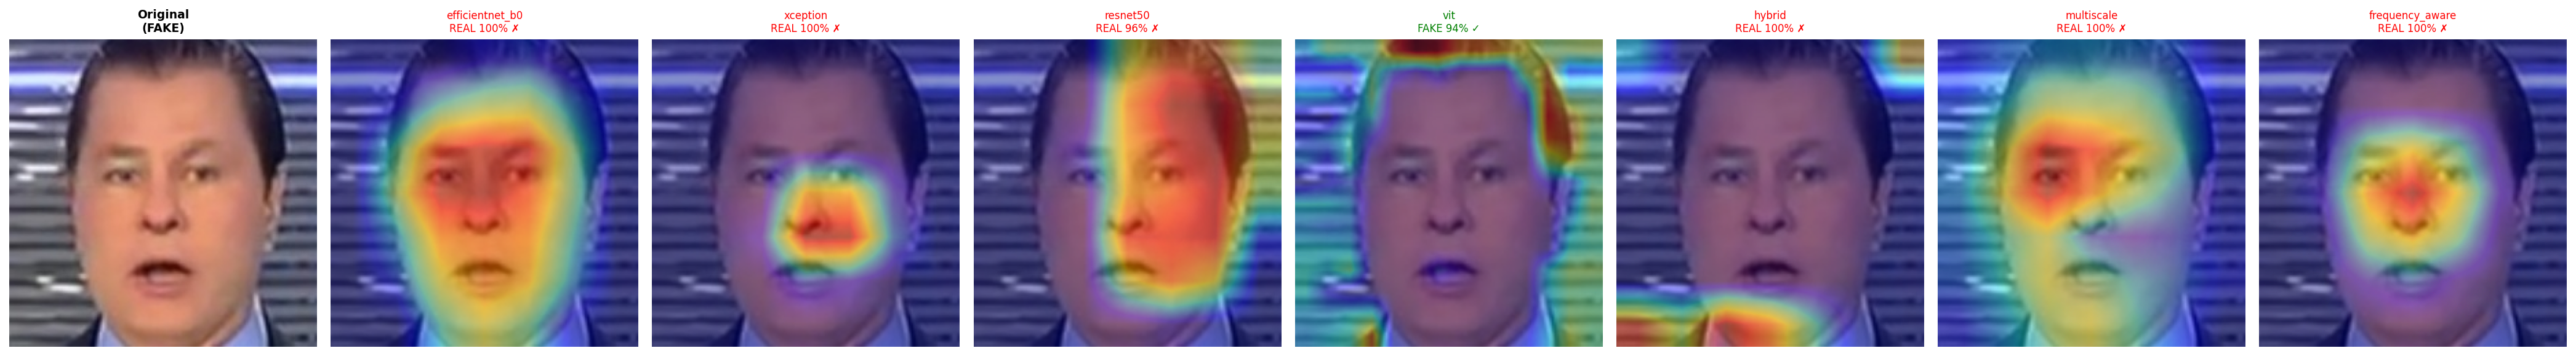
\includegraphics[width=0.45\textwidth]{figures/gradcam_ff_fake.png} \\
(a) Celeb-DF Sample (Real) & (b) FaceForensics++ Sample (Fake --- evaded 6/7 models)
\end{tabular}
\caption{Failure analysis. (a) On in-distribution real images, all CNN models agree unanimously while ViT misclassifies with high confidence. (b) A representative FF++ fake image that successfully evaded 6 out of 7 models---only ViT detected it correctly, validating ViT's superior cross-dataset generalization.}
\label{fig:gradcam_failure}
\end{figure*}

The systematic failure analysis uncovered critical patterns:
\begin{itemize}
    \item \textbf{In-distribution:} All CNNs (6/6 models with CNN components) achieved 10/10 correct classifications on Celeb-DF samples. The ViT scored only 5/10, misclassifying all 5 real Celeb-DF images as fake.
    \item \textbf{Cross-dataset:} On FF++ samples, 14 out of 20 images produced inter-model disagreement. ResNet50 emerged as the most robust single model on this sample (7/10 correct), followed by the Hybrid, Multi-Scale, and Frequency-Aware models (each 6/10).
    \item \textbf{Universal blindspots:} 3 specific FF++ fake images successfully evaded 6 out of 7 models simultaneously. Only the ViT consistently detected these---further confirming ViT's structural advantage for cross-dataset generalization despite its lower in-distribution accuracy.
\end{itemize}

\section{Discussion}
The experimental results reveal several critical insights:
\begin{enumerate}
    \item \textbf{The Accuracy-Robustness Tradeoff:} Models optimized for maximum in-distribution accuracy (EfficientNet, Frequency-Aware CNN) are operationally fragile. A deployed detector must prioritize robustness over benchmark scores.
    \item \textbf{Ensemble Limits:} While ensembling pushed in-distribution performance to 99.51\%, it provided negligible cross-dataset improvement ($<$3\% over single models). Diversity in ensemble members does not compensate for shared inductive biases rooted in spatial feature extraction.
    \item \textbf{Spectral Features Are Distribution-Specific:} The Frequency-Aware CNN's spectral signatures proved specific to Celeb-DF's generation pipeline rather than universally applicable GAN fingerprints.
    \item \textbf{Architectural Topology Dictates Adversarial Fate:} The three-tier adversarial response pattern (collapse, resilience, immunity) maps directly to architectural primitives: standard convolutions are maximally vulnerable, depthwise separable convolutions provide structural resistance, and self-attention provides immunity. This suggests adversarial robustness is an emergent architectural property, not a training artifact.
    \item \textbf{ViT's Dual Nature:} The ViT simultaneously exhibits the lowest in-distribution accuracy (90.54\%) yet the highest cross-dataset accuracy (66.06\%) and complete adversarial prediction invariance. However, its near-random AUC (49.26\%) and systematic misclassification of all real images as fake indicate this invariance likely stems from gradient masking rather than true semantic robustness. Future work should verify this via gradient-free attacks (e.g., SPSA) or black-box transfer attacks to disentangle architectural robustness from degenerate classification behavior.
\end{enumerate}

\section{Conclusion}
This study demonstrates that conventional deepfake detection benchmarking is fundamentally misleading. While the Frequency-Aware CNN (99.84\% AUC) and Soft-Voting Ensemble (99.51\% accuracy) establish new in-distribution bounds, these gains do not transfer: all CNN-based architectures collapse under adversarial perturbations and fail to generalize across datasets. For real-world forensic deployment, it is recommended to use architectures built around ViT and XceptionNet cores, prioritizing operational robustness over peak benchmark accuracy. Future work should investigate adversarial training to elevate the robustness floor, temporal detection via Video Transformers, and universal spectral signatures applicable across generation methods.

\section*{Acknowledgment}
The authors thank the research teams who created and maintained the Celeb-DF and FaceForensics++ datasets for enabling reproducible deepfake detection research.

\begin{thebibliography}{00}
\bibitem{cross_dataset} Y. Li, X. Yang, P. Sun, H. Qi, and S. Lyu, ``Celeb-DF: A large-scale challenging dataset for deepfake forensics,'' in Proc. IEEE/CVF CVPR, 2020, pp. 3207--3216.
\bibitem{faceforensics} A. R\"ossler, D. Cozzolino, L. Verdoliva, C. Riess, J. Thies, and M. Nie{\ss}ner, ``FaceForensics++: Learning to detect manipulated facial images,'' in Proc. IEEE/CVF ICCV, 2019, pp. 1--11.
\bibitem{xception} F. Chollet, ``Xception: Deep learning with depthwise separable convolutions,'' in Proc. IEEE CVPR, 2017, pp. 1251--1258.
\bibitem{efficientnet} M. Tan and Q. Le, ``EfficientNet: Rethinking model scaling for convolutional neural networks,'' in Proc. ICML, 2019, pp. 6105--6114.
\bibitem{resnet} K. He, X. Zhang, S. Ren, and J. Sun, ``Deep residual learning for image recognition,'' in Proc. IEEE CVPR, 2016, pp. 770--778.
\bibitem{vit} A. Dosovitskiy et al., ``An image is worth 16x16 words: Transformers for image recognition at scale,'' in Proc. ICLR, 2021.
\bibitem{frequency_analysis} F. Marra, D. Gragnaniello, D. Cozzolino, and L. Verdoliva, ``Detection of GAN-generated fake images over social networks,'' in Proc. IEEE MIPR, 2018, pp. 384--389.
\bibitem{fgsm} I. J. Goodfellow, J. Shlens, and C. Szegedy, ``Explaining and harnessing adversarial examples,'' in Proc. ICLR, 2015.
\bibitem{pgd} A. Madry, A. Makelov, L. Schmidt, D. Tsipras, and A. Vladu, ``Towards deep learning models resistant to adversarial attacks,'' in Proc. ICLR, 2018.
\end{thebibliography}

\end{document}
